% Fig. 1 v4: one SafeLIBERO episode, prior safety layer (left) vs AG3S (right). Layout after the user's figurelabs mock.
% Source: paper/figures/fig01_teaser/v4/fig01_v4.pdf (+ fig01_v4.json: per-panel run, frame, crop, sha256, overlay definition).
% Scripts: paper/tools/plotting/fig1_v4_assets.py (recorded frames + recorded geometry), cvpr_v4_fig1_compose.py.
\begin{minipage}{\textwidth}
\centering
\captionsetup{type=figure,hypcap=false}
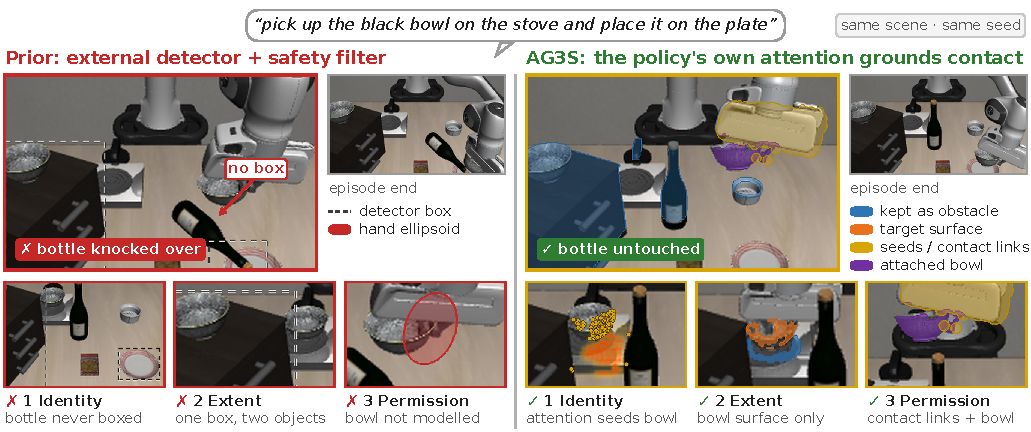
\includegraphics[width=\textwidth]{../figures/fig01_teaser/v4/fig01_v4.pdf}
\caption{\textbf{Same scene, same seed: a prior safety layer guards what its detector boxed; \sys\ guards everything but the surface the policy is about to grasp.}
SafeLIBERO Level~I, wine bottle as obstacle, frozen $\pi_{0.5}$. \emph{Left:} AEGIS~\cite{hu2026vlsa} keeps the end effector away from detected objects, but the open-vocabulary detector boxes the cabinet and the plate and never the bottle, so the bottle is knocked over at the same moment as without any safety layer (main frame and episode end).
Insets: (1) the bottle has no box; (2) one box spans the cabinet and the bowl on it; (3) KNOWS$^\ast$~\cite{park2026knows} models the robot as a single end-effector ellipsoid (red), so a carried bowl is not modelled.
\emph{Right:} with \sys, every observed surface stays an obstacle (blue), the carried bowl is attached geometry (purple) and only the hand's contact links (gold) may touch it; the bottle stays upright and the bowl is placed.
Insets: (1) the policy's noun attention, lifted to the observed points, seeds the bowl (gold); (2) depth continuity bounds the bowl's surface (orange) and keeps the adjacent geometry (blue); (3) contact links and the attached bowl while carrying.
All panels are recorded frames of one episode per method, or recorded geometry drawn onto them.}
\label{fig:teaser}
\end{minipage}
